\documentclass[UTF8]{article}
\usepackage{ctex}
\usepackage{amsmath}
\usepackage{graphicx}

\begin{document}
\section{简谐振动}
\subsection{简谐振动的定义}

    一、振动的定义及分类

    1.定义:一个物理量在某一定值附近往复变化,该物理量的运动形式成为振荡

    \;\;特征:存在平衡位置+具有周期性

    2.分类:按物理量类型划分:电磁振荡+机械振动

    \;\;在某一空间位置附近做来回往复的周期运动的物体做机械振动

    \;\;按受力或能量转换划分:自由振动(无阻尼振动,阻尼振动)+受迫振动

    根据机械振动的定义可知,机械振动的运动方程可以用周期函数来描述$f(t) = f(t+T)$

    任何一个复杂的振动均可分解为若干个以正(余)弦形式运动的振动
    \\

    二、简谐运动的定义

    1.定义:物体运动时,物体相对于平衡位置的位移按余弦(正弦)函数的规律随时间变化,这样的振动称为简谐振动,又称为谐振动。
    简谐运动是最简单、最基本的振动。

    2.模型:弹簧振子(线性谐振动)模型 = 轻弹簧 + 平动刚体

    3.运动方程:$x = Acos(\omega t + \phi_0)$,$A$振幅,$\omega$原频率,$\phi_0$初相位

\subsection{简谐运动的基本特征}

    一、两个理想化模型

    1.弹簧振子

    受力分析:$F = -kx$

    由牛顿第二定律,得:
    \[-kx = ma = m\frac{d^2x}{dt^2}\;\;\;\mbox{其中:}\frac{k}{m} = \omega^2\]

    动力学微分方程:
    \[\frac{d^2x}{dt^2} + \omega^2 x = 0\;\;\;\mbox{其中:}\frac{k}{m} = \omega^2\]

    运动学方程(振动方程):
    \[x = Acos(\omega t + \phi_0)\]

    2.单摆(小角度)

    受力分析:$M = -mgl\theta$

    由转动定律,有:
    \[M = J\beta = ml^2\frac{d^2\theta}{dt^2}\;\;\;\mbox{其中:}\frac{g}{l} = \omega^2\]

    动力学微分方程:
    \[\frac{d^2\theta}{dt^2} + \omega^2\theta = 0\;\;\;\mbox{其中:}\frac{g}{l} = \omega^2\]

    运动学方程(振动方程):
    \[\theta = \theta_0cos(\omega t + \phi_0)\]

    二、简谐运动的判定

    1.物体只受线性恢复力作用
    \[F = -kx\mbox{或}M= -k\theta\]

    2.动力学方程满足
    \[\frac{d^2x}{dt^2} + \omega^2x = o\]

    3.在无外来强迫力作用下,质点离开平衡位置的位移是时间的正弦函数或余弦函数
    \[x = Acos(\omega t + \phi_0)\]

    判断一振动是否是简谐振动用三种定义中任何一种皆可

    三、简谐运动的速度和加速度

    动力学方程:
    \[\frac{d^2x}{dt^2} = -\omega^2 x\]

    解方程得:
    \[x = Acos(\omega t + \phi)\;\;\;A,\phi\mbox{是积分常数,根据初始条件确定}\]

    速度:
    \[v = \frac{dx}{dt} = -A\omega sin(\omega t + \phi)\]

    加速度:
    \[a = \frac{d^2x}{dt^2} = -A\omega^2cos(\omega t + \phi) = -\omega^2x\]

\subsection{描述简谐运动的物理量}

    1.振幅A:与振动系统初始运动状态和系统属性有关,反应能量大小。
    \[A = \sqrt{x_0^2 + \frac{v_0^2}{\omega^2}}\]

    2.圆(角)频率$\omega$:由系统本身属性决定的常数,与初始条件无关(固有角频率)

    周期:$T = \frac{2\pi}{\omega}$,物体完成一次全振动所经历的时间,[SI]:s

    频率:$\nu = \frac{1}{T} = \frac{\omega}{2\pi}$,单位时间内质点完成的全振动的次数,[SI]:Hz

    角频率:$\omega = 2\pi\nu$,描述谐振运动的频率和周期,[SI]:$rad\cdot s^{-1}$

    3.相位$\omega t + \phi_0$,初相$\phi_0$

    (1)初相位:$\phi_0$,描述t=0时刻的运动状态
    \[\phi_0 = arctan(-\frac{v_0}{\omega x_0})\]

    (2)相位(位相)$\omega t + \phi$的物理意义:反应系统振动状态,运动状态变化趋势,比较频率相同的两振动系统的振动步调

\subsection{简谐运动的表示方法}

    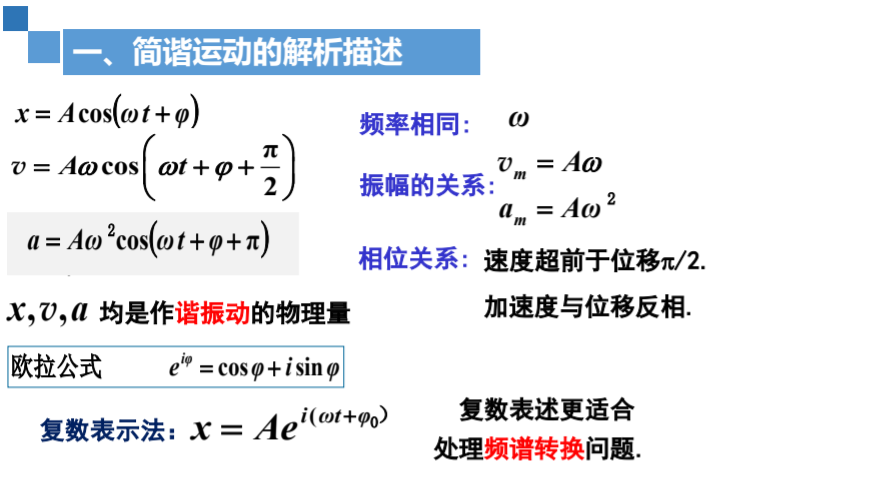
\includegraphics[width=13cm, height=8cm]{D:/UniversityNote/PhyNote/9/901.png}
    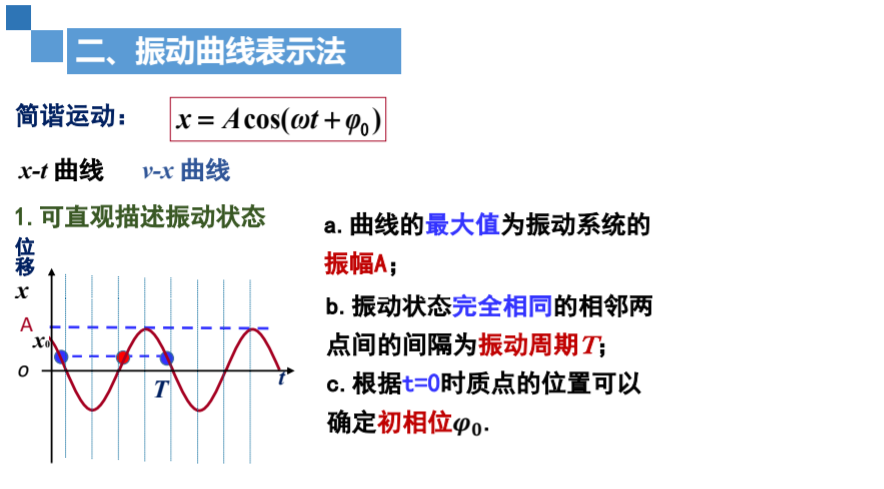
\includegraphics[width=13cm, height=8cm]{D:/UniversityNote/PhyNote/9/902.png}
    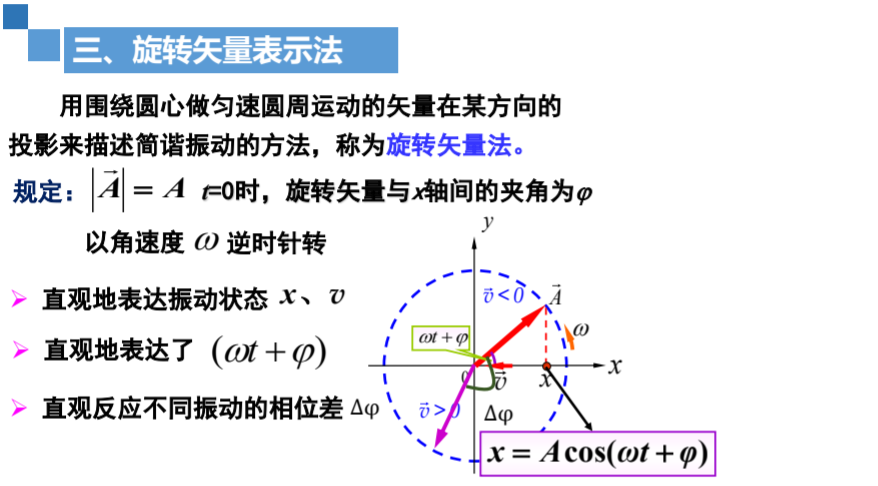
\includegraphics[width=13cm, height=8cm]{D:/UniversityNote/PhyNote/9/903.png}

\subsection{简谐运动的能量}

    1.谐振动系统的动能:
    \[E_k = \frac{1}{2}mv^2 = \frac{1}{2}m\omega^2 A^2sin^2(\omega t + \phi_0)\]

    2.谐振动系统的势能:
    \[E_p = \frac{1}{2}kx^2 = \frac{1}{2}kA^2cos^2(\omega t + \phi_o)\;\;\;\mbox{考虑到:}\frac{k}{m}\omega^2\]

    3.谐振动系统的总能量:
    \[\mbox{孤立谐振动系统机械能守恒:}E = E_k + E_p = \frac{1}{2}kA^2\]

    4.动能和势能的变化频率是位移变化频率的2倍,总能量并不改变。

    5.能量方法是工程中求振动系统固有频率是常用的方法:

    由振动过程中机械能守恒:
    \[E = \frac{1}{2}mv^2 + \frac{1}{2}kx^2 = \mbox{常数}\]

    两边求导:
    \[mv\frac{dv}{dt} + kx\frac{dx}{dt} = 0\Longrightarrow m\frac{d^2x}{dt^2} + kx = 0\Longrightarrow \omega^2 = \frac{k}{m}\]

\subsection{简谐运动的合成}
\subsubsection{同方向同频率简谐运动的合成}

    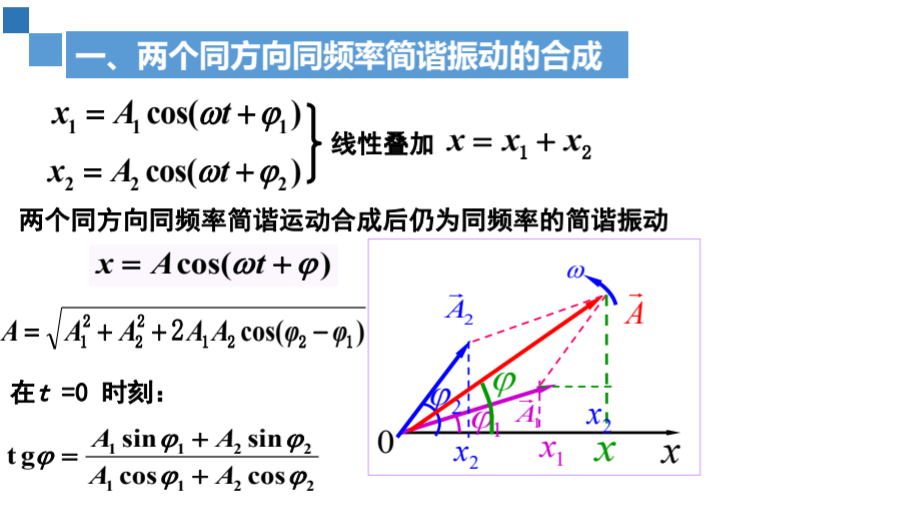
\includegraphics[width=13cm, height=8cm]{D:/UniversityNote/PhyNote/9/904.png}
    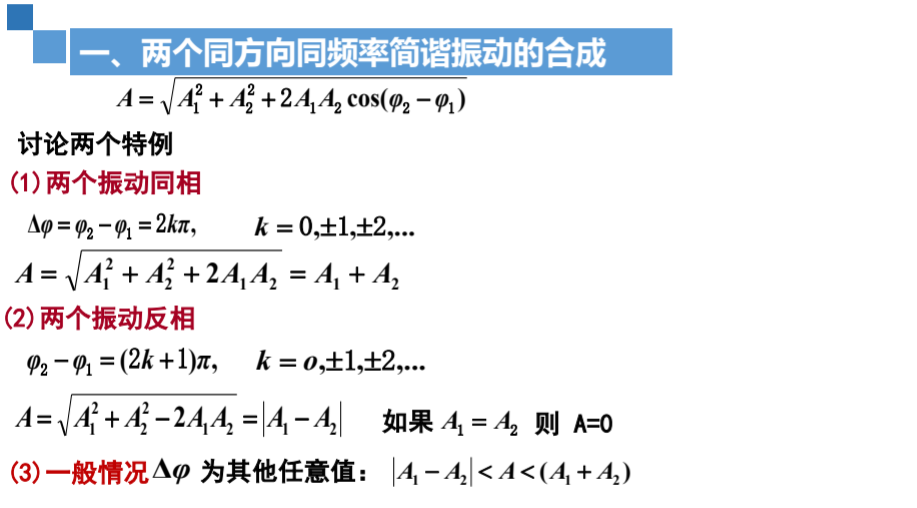
\includegraphics[width=13cm, height=8cm]{D:/UniversityNote/PhyNote/9/905.png}
    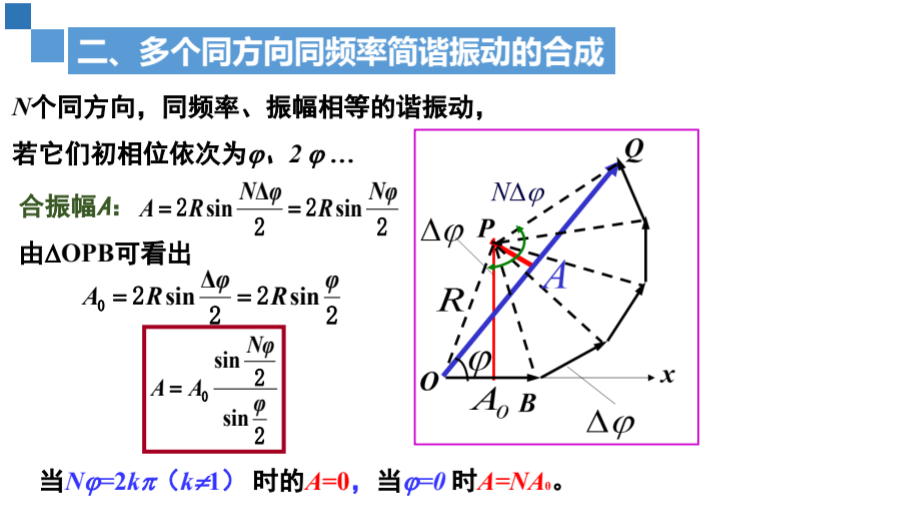
\includegraphics[width=13cm, height=8cm]{D:/UniversityNote/PhyNote/9/906.png}

\subsubsection{同方向不同频率简谐振动的合成}

    若$\omega_1 = \omega_2$,则$\Delta \phi$不变;同方向同频率两个简谐运动的合成仍为简谐运动

    若$\omega_1 \neq \omega_2$,则$\Delta \phi$变;同方向不同频率的两个简谐运动搞的合成为一复杂运动

    同方向不同频率简谐振动的合成:
    \[x_1 = Acos\omega_1 t\;\;\;x_2 = Acos\omega_2 t\mbox{振幅相同,初相为零}\]

    \[x = x_1 + x_2 = Acos\omega_1 t + Acos\omega_2 t = 2Acos\frac{(\omega_2 - \omega_1)t}{2}cos\frac{(\omega_2 + \omega_1)t}{2}\]

    当$\omega_1 - \omega_2<<\omega_1\; or \;\omega_2$时,振幅随时间的变化非常缓慢

    拍:频率较大而频率差较小的两个同方向简谐振动合成时,其和振动的振幅时而增强时而减弱的现象

    拍频:单位时间内合成振幅加强(减弱)的次数
    \[\nu_{\mbox{拍}} = \vert \frac{\omega_2 - \omega_1}{2\pi} \lvert = \vert \nu_2 - \nu_1 \lvert\]

\subsection{互相垂直的谐振动的合成}

    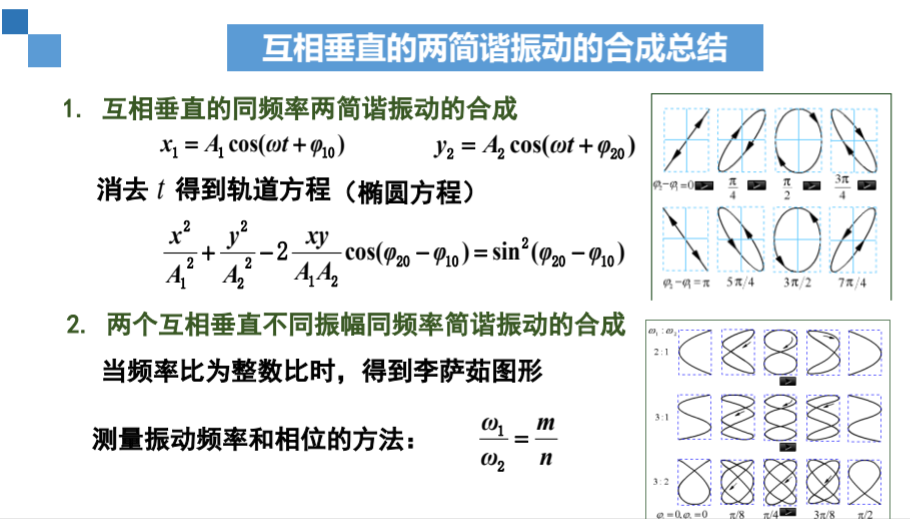
\includegraphics[width=13cm, height=8cm]{D:/UniversityNote/PhyNote/9/907.png}

\end{document}